\documentclass{article}
\usepackage{calc, amsmath, amssymb, amsfonts, amsthm, mathtools, empheq}
\usepackage{tabularx,colortbl}
\usepackage{fancyhdr, graphicx}
\graphicspath{{figures/}}
%\usepackage{algorithm}
\usepackage{algpseudocode}
\usepackage{framed}
\usepackage{enumerate}
\usepackage{subcaption}
\usepackage{hyperref}
\usepackage{cite}
\usepackage[numbers]{natbib}
\usepackage[]{algorithm2e}
\usepackage{listings}
\usepackage{color}
\definecolor{dkgreen}{rgb}{0,0.6,0}
\definecolor{gray}{rgb}{0.5,0.5,0.5}
\definecolor{mauve}{rgb}{0.58,0,0.82}

\lstset{ %
 language=Matlab,                % the language of the code
 basicstyle=\footnotesize,           % the size of the fonts that are used for the code
 showstringspaces=false,
 tabsize=2,                      % sets default tabsize to 2 spaces                
 keywordstyle=\color{blue},          % keyword style
 commentstyle=\color{dkgreen},       % comment style
 stringstyle=\color{mauve},         % string literal style
}


% Homework Data:
% HW Title:
\newcommand{\hwkTitle}{Homework 5: Uncertainty Planning}
% Homework Date:
\newcommand{\hwkDate}{03/07/2014}
% My name!
\newcommand{\hwkAuthor}{Vishnu Desaraju, Nitish Thatte, Bhaskar Vaidya}
% Class name:
\newcommand{\hwkClass}{16-899C: ARCL}

% Margins:
\topmargin=-0.45in
\evensidemargin=0in
\oddsidemargin=0in
\textwidth=6.5in
\textheight=9.0in
\headsep=0.25in

% Header & Footer
\pagestyle{fancy}
%\lhead{}
%\chead{}
%\rhead{\hwkDate}
\lfoot{\hwkDate}
\cfoot{}
%\cfoot{\hwkClass\ - \hwkTitle}
\rfoot{Page\ \thepage}
\renewcommand\headrulewidth{0.4pt}
\renewcommand\footrulewidth{0.4pt}

%%%%%%
% Extra (Awesome) Functions:
%%%%%%

% Boxes & Centers solution. 
% Usage: \soln{This is the solution.}
\newcommand{\soln}[1]{ \begin{center} \fbox{#1} \end{center}}

% Inserts a number in scientific notation. 
% Usage: <mantissa>\e{<exponent>}
\providecommand{\e}[1]{\ensuremath{\times 10^{#1}}}

% Adds a degree symbol. Usage: <temperature>\degree C
\newcommand{\degree}{\(^\circ\)}

% Adds a partial differential fraction. Usage: \dd{V}{T} % For dV/dT
\newcommand{\dd}[2]{\ensuremath{\frac{\partial #1}{\partial #2}}}
% Adds norm. Usage\norm{stuff}
\newcommand{\norm}[1]{\lVert#1\rVert}
\newcommand{\ip}[2]{\left\langle #1,\ #2\right\rangle}
\newcommand{\paren}[1]{\left( #1 \right)}
\newcommand{\abs}[1]{\left| #1 \right|}

\def\ci{\perp\!\!\!\perp}

\newcommand{\bldsym}[1]{\boldsymbol{#1}}


% for argmin
\DeclareMathOperator*{\argmin}{arg\,min}
\DeclareMathOperator*{\argmax}{arg\,max}


\newcommand{\problem}[1]{\hfill \vspace{2ex} \\ \textbf{\large{#1}} \vspace{2ex} \newline}
\newcommand{\question}[1]{\hfill \\ \textbf{#1} \hfill \\ \indent}

\newlength\dlf
\newcommand{\alignedbox}[2]{
  % #1 = before alignment
  % #2 = after alignment
  &
  \begingroup
  \settowidth\dlf{$\displaystyle #1$}
  \addtolength\dlf{\fboxsep+\fboxrule}
  \hspace{-\dlf}
  \boxed{#1 #2}
  \endgroup
}
\newcommand{\insertTitle}{\begin{center}\LARGE{\hwkClass\ - \hwkTitle} \\ \large{\hwkAuthor} \end{center}}

\title{\hwkTitle\ -\ \hwkClass}
\author{\hwkAuthor}
\date{Sep. 17, 2013}

%%%%%%%%%%%%%%%%%%%%%%%%%%%%%%%%%%%%%%%%%%%%%%%%%%%%%%%%%%%%%%%%%%%%%%%%%%%%%%%%

\begin{document}
\insertTitle
\vspace*{3ex}

\section{Planning Algorithm: A-Star}

We decided to use the A-Star search algorithm to solve the planning problem. Our nodes were $(x, y, \theta)$ tuples, and we utilized a small set of grid-based motion primitives as our edges. We hand-tuned the number and curvature of the motion-primitives to obtain a good tradeoff between planning time and ability to solve complex geometries.

\subsection{Motion Primitives and Cost}

Our motion primitives were designed as short Dubin's curves, designed to be less than 9 meters in length. While the model is not actually a Dubin's car, the hope was that Dubin's curves would be close enough to dynamically feasible to be able to track well with a simple controller. In order to generate these primitives, we instantiated a $3x3 m$ grid with a spacing of $1 m$, and computed Dubin's curves from the origin $(0,0)$ to each of the grid points. Each primitive could only start at a heading of $0$ and end at a heading of increments of $\frac{\pi}{4}$, ensuring that the search space of nodes is finite. Due to the max turn radius constraint implemented in the Dubin's curve solver ($3 m$), some of the curves contained one or more loops, which was undesirable in a primitive. Thus, we only added Dubin's curves with no loops (by thresholding the curve length) to the primitive library.

Due to the structure of the problem, backwards motions could have been necessary to reach the goal. We implemented several backwards primitives, each beginning and ending with a heading of $0$, and with lengths of 1 m, 1.5 m, 2.0 m, 2.5 m, 3.0 m, and 3.5 m. These motions completed our primitive library, shown superimposed in Fig. \ref{fig:prim_lib}.


During A-Star, when we expand a node, we translate and rotate each primitive in the library to the position and orientation of the end of the node's primitive, thus generating the node's children. We then check the children for collisions with obstacles, and add the valid ones to the priority queue. The cost associated with each primitive is simply the length of the curve, which makes the cost of a node the total path length to get to that node.

\begin{figure}[ht]
\centering
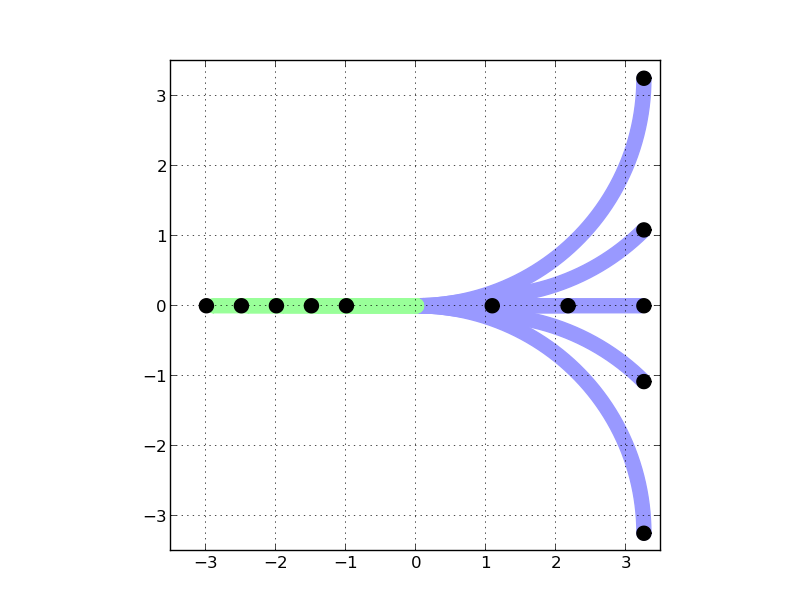
\includegraphics[width=256pt,keepaspectratio]{figures/primitives.png}
\caption{Primitive Library}
\label{fig:prim_lib}
\end{figure}

\subsection{Heuristic}

In order to come up with a admissible heuristic, we run value iteration on an MDP in the discretized world, where the actions are straight-line motions on an 8-connected grid, and the cost of each action is the length of the action. Example heuristics are shown in Fig. \ref{fig:valuefcns}.
 
\begin{figure}[ht]
    \centering
    \begin{subfigure}[b]{0.45\textwidth}
        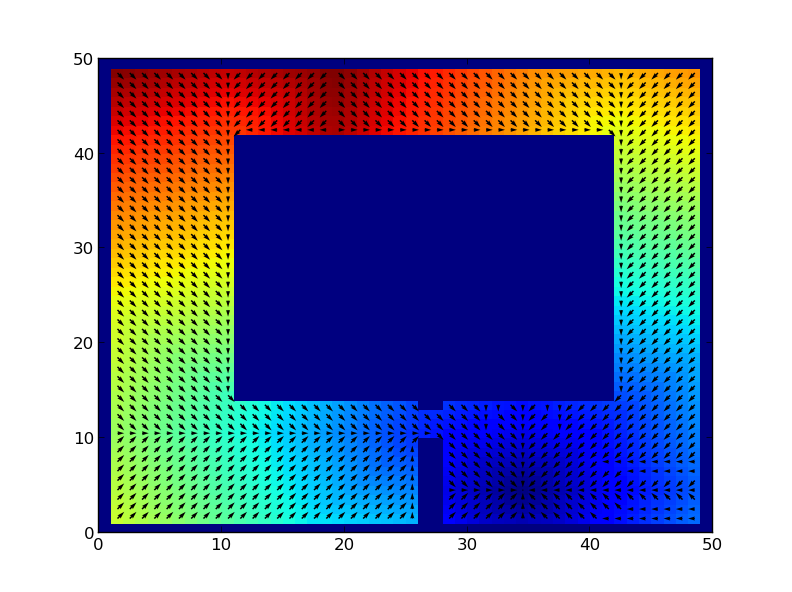
\includegraphics[width = \textwidth]{map1value.png}
        \caption{Map 1 Heuristic}
        \label{fig:map1value}
    \end{subfigure}
    \begin{subfigure}[b]{0.45\textwidth}
        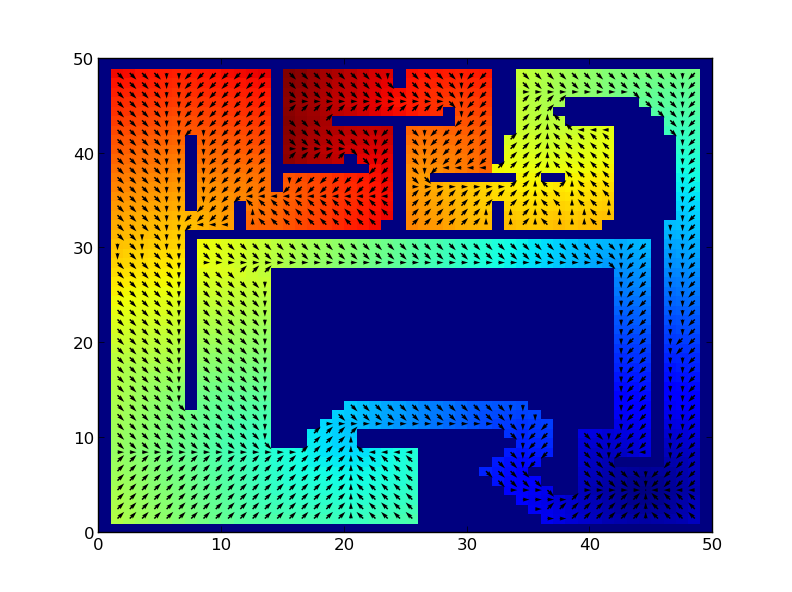
\includegraphics[width = \textwidth]{map2value.png}
        \caption{Map 2 Heuristic}
        \label{fig:map2value}
    \end{subfigure}
    \begin{subfigure}[b]{0.45\textwidth}
        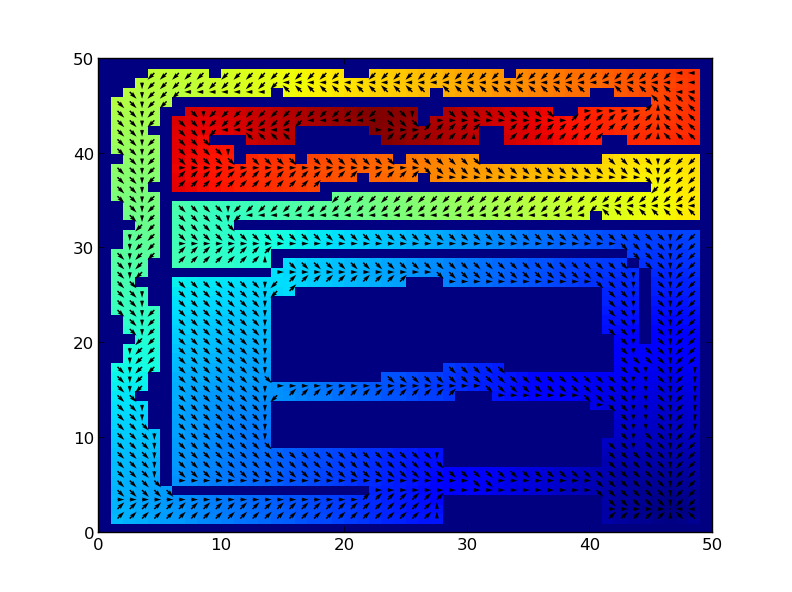
\includegraphics[width = \textwidth]{map3value.png}
        \caption{Map 3 Heuristic}
        \label{fig:map3value}
    \end{subfigure}
    \caption{Freespace value functions and policies for inscribed disk model}
    \label{fig:valuefcns}
\end{figure}

\subsection{Dealing with Uncertainty}

In order to take into account the stochastic nature of the problem, we modify our heuristic to include uncertainty. The intuition for doing this is to weight the heuristic of uncertain nodes proportional to uncertainty of openness, so that the planner stays away from locations very likely to be bridges. We implement this by adding a state-dependent cost to the MDP; if a state is within the observation radius of the grid, the associated cost is its distance from the starting location (the robot's current location). Example modified heuristics are shown in Fig. \ref{fig:valuefcns_mod}; as can be seen from these figures, the value function is now heavily dependent on the uncertainty in the bridges. The decision point for the value function (point of zero gradient) changes when the uncertainty is added. We can see from the comparison of Fig. \ref{fig:valuefcns} and Fig. \ref{fig:valuefcns_mod} that the decision point moves in a way that makes the gradient in more states descend towards the path least likely to be blocked.

\begin{figure}[ht]
    \centering
    \begin{subfigure}[b]{0.45\textwidth}
        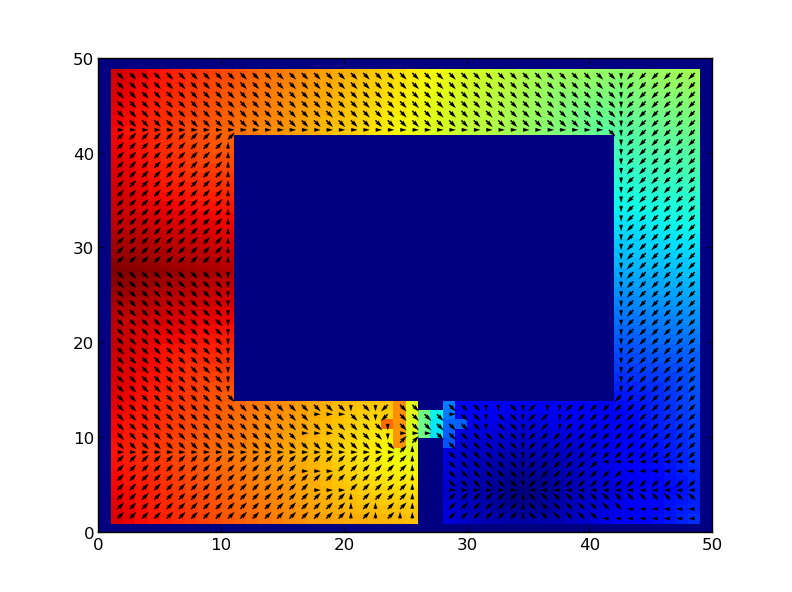
\includegraphics[width = \textwidth]{map1value_uncertain.png}
        \caption{Map 1 Heuristic Under Uncertainty}
        \label{fig:map1value_mod}
    \end{subfigure}
    \begin{subfigure}[b]{0.45\textwidth}
        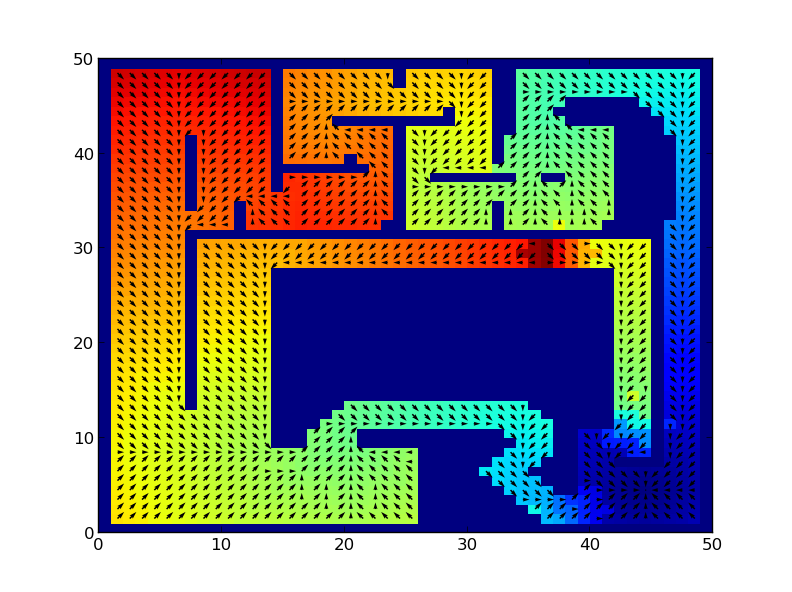
\includegraphics[width = \textwidth]{map2value_uncertain.png}
        \caption{Map 2 Heuristic Under Uncertainty}
        \label{fig:map2value_mod}
    \end{subfigure}
    \begin{subfigure}[b]{0.45\textwidth}
        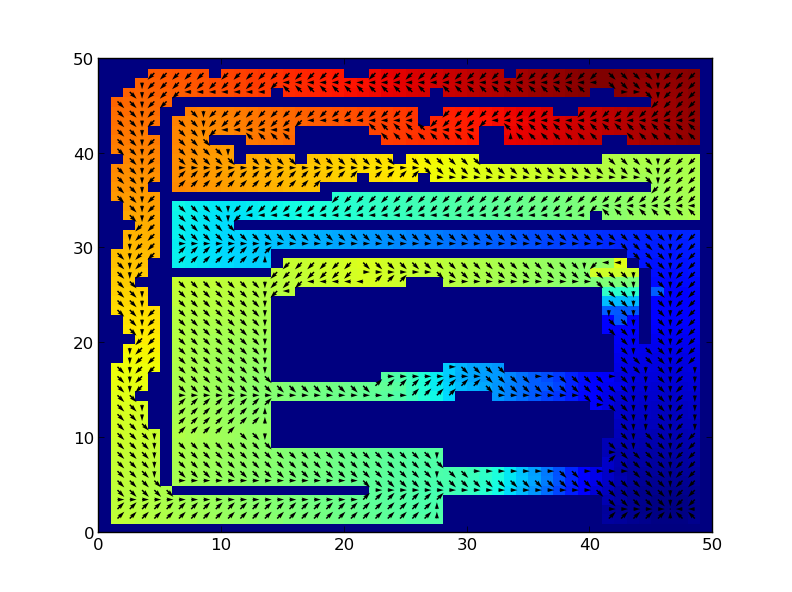
\includegraphics[width = \textwidth]{map3value_uncertain.png}
        \caption{Map 3 Heuristic Under Uncertainty}
        \label{fig:map3value_mod}
    \end{subfigure}
    \caption{Modified value functions and policies for inscribed disk model}
    \label{fig:valuefcns_mod}
\end{figure}

While modifying the heuristic may make it inadmissible, experimental validation has shown that the planner can find paths through the test paths fairly fast.


\section{Replanning and Control}

Due to the fact that we only discover whether a bridge is blocked or not when the robot approaches within the observation distance of the bridge, replanning is a necessary part of the system architecture. When we make an observation, we check whether out current plan has been invalidated; if so, we first run value iteration to recompute the heuristic, and then recompute a plan using A-Star, using our current position and heading as the initial node.

Due to the fact that our motion primitives are not dynamically feasible, we implemented a controller to track the trajectory correctly. We implemented a switching controller, with three different modes, as shown below:

\begin{align*}
u =
\begin{cases}
sat(-k_P\,e_1 - k_D\,\dot{e_1} + \theta_{ref},\; -1,\; 1) & \text{Forward Motion}\\
sat(-k_P\,e_2,\; -1,\; 1) & \text{End of Forward Motion}\\
-2 & \text{Reverse}
\end{cases}
\end{align*}
where 
\begin{align*}
\centering
e_1 &= \theta - \arctan{\frac{y_{ref} - y}{x_{ref} - x}}\\
e_2 &= \theta - \theta_{ref}
\end{align*}

This controller tracks trajectories primitive by primitive, only transitioning to the next primitive when at the end of the current one. We do this tracking by `carrot following', controlling to a point 0.9 m ahead of the robot on the trajectory. At the end of the primitive, we switch to an angle alignment controller, which correctly aligns us with the heading of the final waypoint on the primitive. This mitigates any error in our third control mode, which is just open loop reverse of the robot. Reversing can lead to diverging from the desired trajectory if the initial heading is even slightly off from the final heading, which motivates using the heading-approach controller right before the end of the trajectory.

\section{Results}

We ran several trials on each of the seven maps given, sampling the seed map distribution to get a ground truth map. We computed statistics on average number of collisions, failed plans, successes, runtime, and path length. Our results are shown below: 
\vspace{24pt}\\
\begin{tabular}{|c|c|c|c|c|c|c|c|}
\hline 
• & No. Trials & Failed Planning & Collisions & Successes & Avg. Path Length & Time  \\ 
&&&&&(Success Only)&(Planning+Execution)\\
\hline 
Map 1 & 2 & 0 & 0 & 5 & 96 m & 55 s \\ 
\hline 
Map 2 & 5 & 1 & 0 & 4 & 67 m & 143 s \\ 
\hline 
Map 3 & 5 & 0 & 3 & 2 & 50 m & 122 s\\ 
\hline 
Map 4 & 5 & 1 & 0 & 4 & 54 m & 116 s \\ 
\hline 
Map 5 & 5 & 0 & 2 & 3 & 149 m & 289 s \\ 
\hline 
Map 6 & 5 & 0 & 2 & 3 & 126 m & 238 s \\ 
\hline 
Map 7 & 5 & 3 & 0 & 2 & 67 m & 192 s \\ 
\hline 
\end{tabular} 
\vspace{24pt}
\\
In general, we see that our approach leads the robot to plan paths that are least likely to be blocked. Thus, we perform fairly well on many of the maps. However, in some of the maps with tight corridors, our approach performs poorly due to a small primitive library. An example successful trajectory is given in Fig. \ref{fig:map6good}. We can see the initial plan in Fig. \ref{fig:map61}. This plan avoids areas with a high probability to be blocked, which explains the roundabout route. As the robot encounters obstacles in its path, as shown in Fig. \ref{fig:map61} and Fig. \ref{fig:map62}. Additionally, when the robot passes a bridge that turns out to be closed, it replans and finds a shorter cost path, due to the recomputation of the heuristic (Fig. \ref{fig:map63}). It then finds that the planned route is blocked (Fig. \ref{fig:map64}) and plans and executes its way to the goal (Fig. \ref{fig:map65}).

\newpage

\begin{figure}[ht]
    \centering
    \begin{subfigure}[b]{0.3\textwidth}
        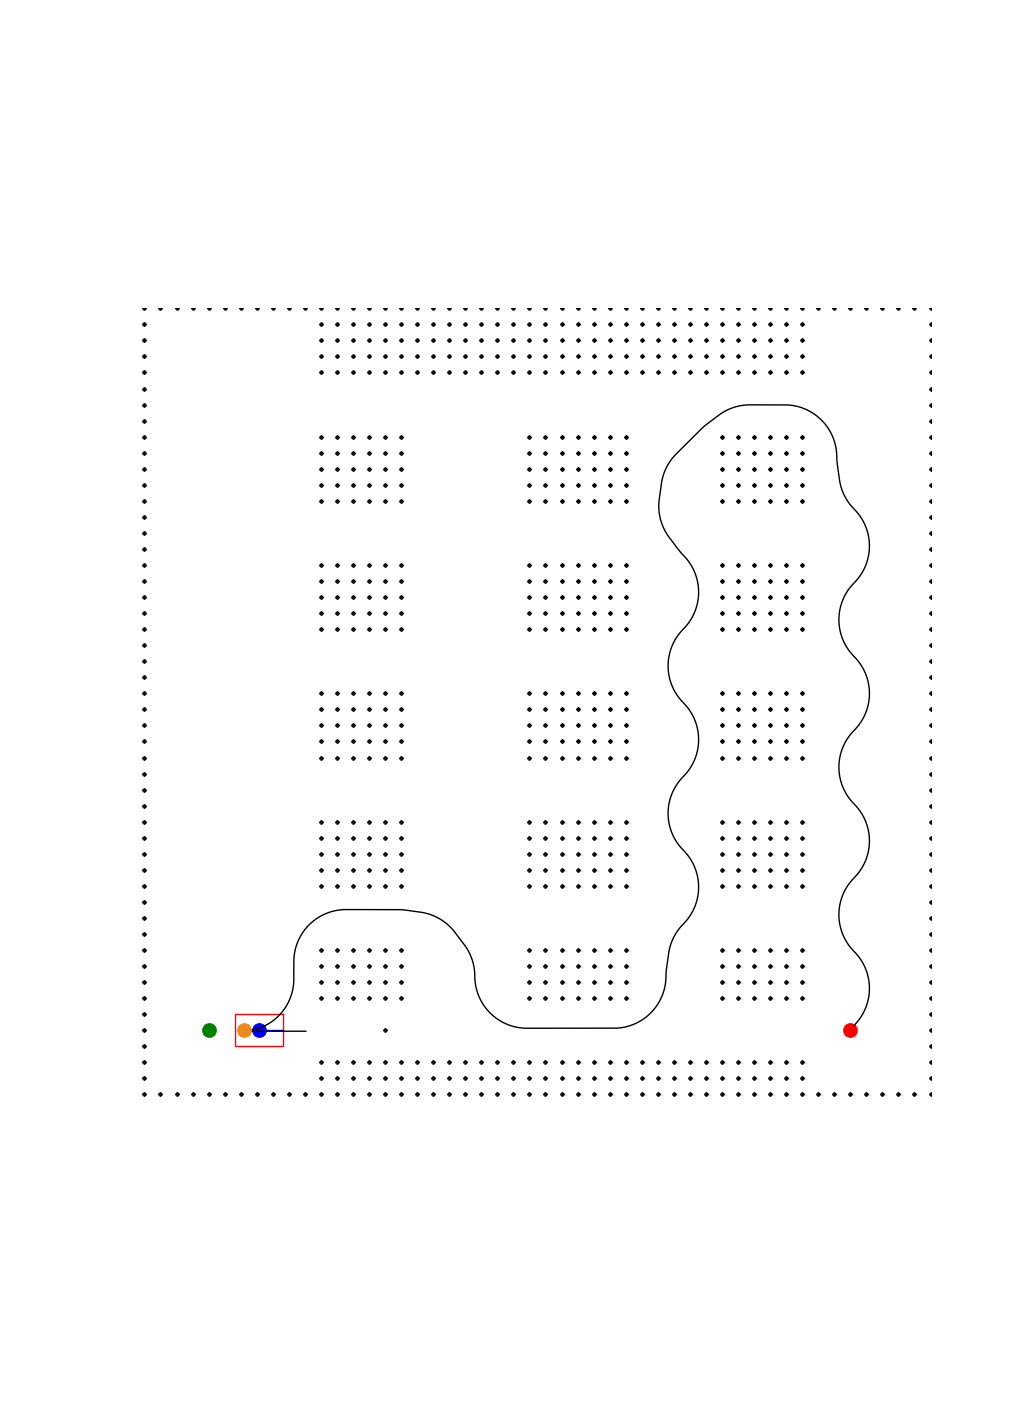
\includegraphics[width = \textwidth]{map6plan2.png}
        \caption{Initial Plan}
        \label{fig:map61}
    \end{subfigure}
    \begin{subfigure}[b]{0.3\textwidth}
        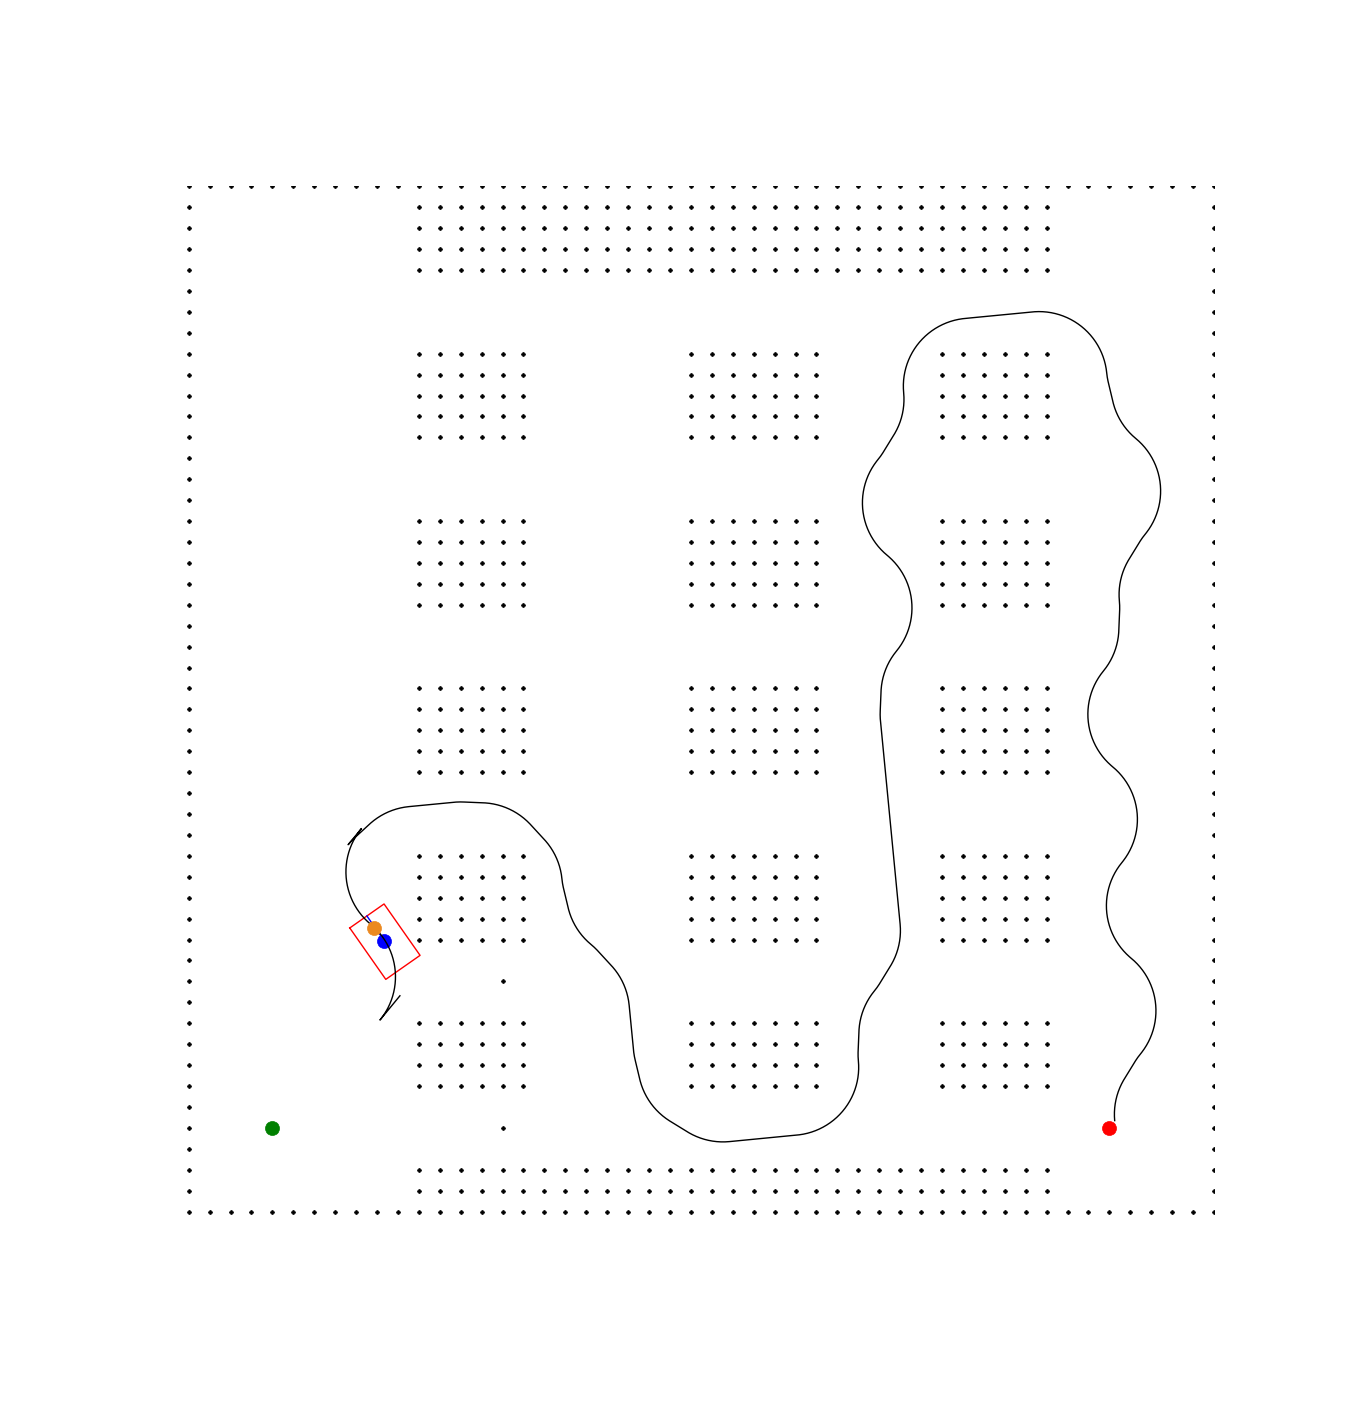
\includegraphics[width = \textwidth]{map6plan3.png}
        \caption{Replan 1}
        \label{fig:map62}
    \end{subfigure}
    \begin{subfigure}[b]{0.3\textwidth}
        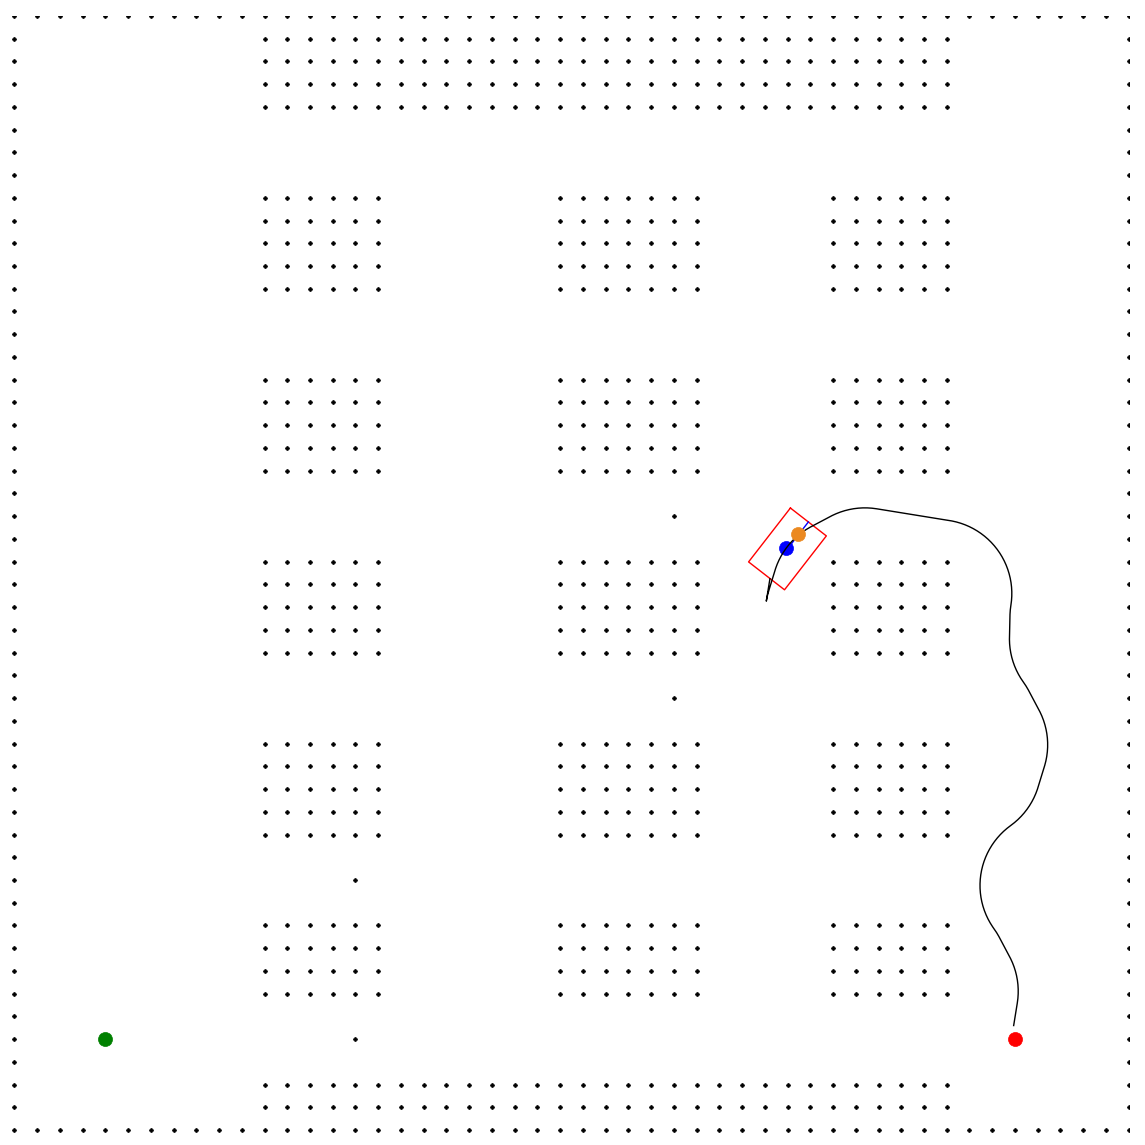
\includegraphics[width = \textwidth]{map6plan3_2.png}
        \caption{Replan 2}
        \label{fig:map63}
    \end{subfigure}
    \begin{subfigure}[b]{0.3\textwidth}
        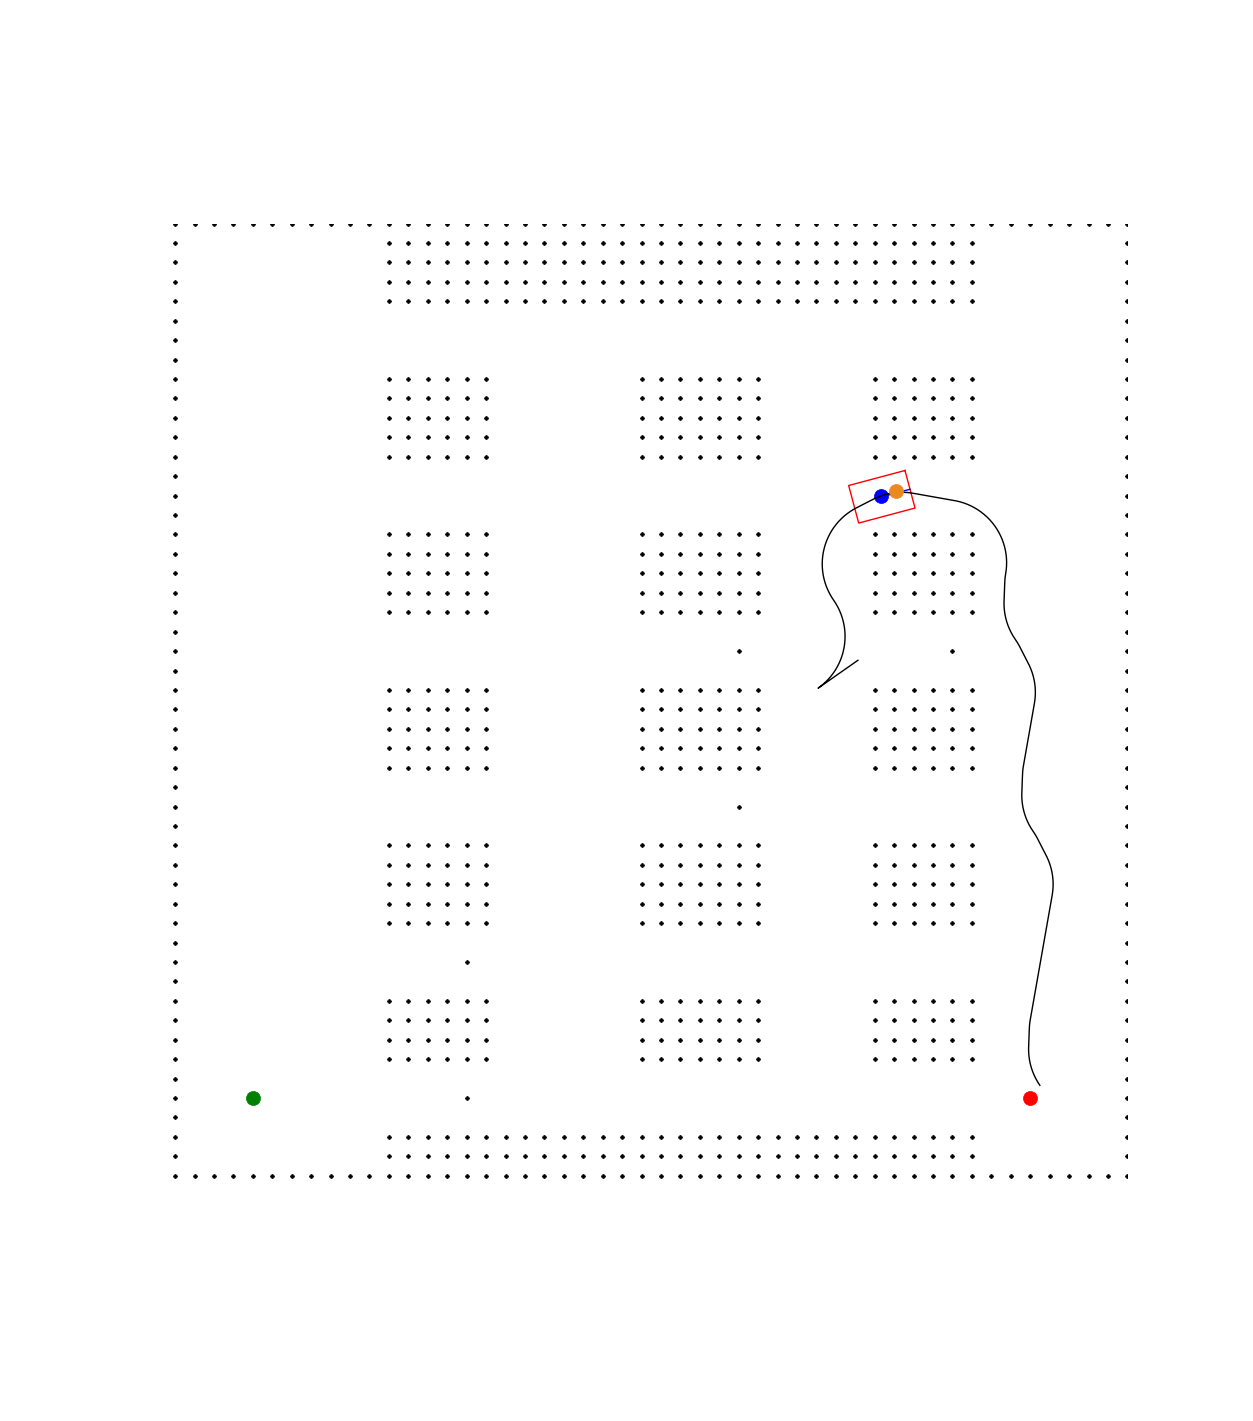
\includegraphics[width = \textwidth]{map6plan3_3.png}
        \caption{Replan 3}
        \label{fig:map64}
    \end{subfigure}
    \begin{subfigure}[b]{0.3\textwidth}
        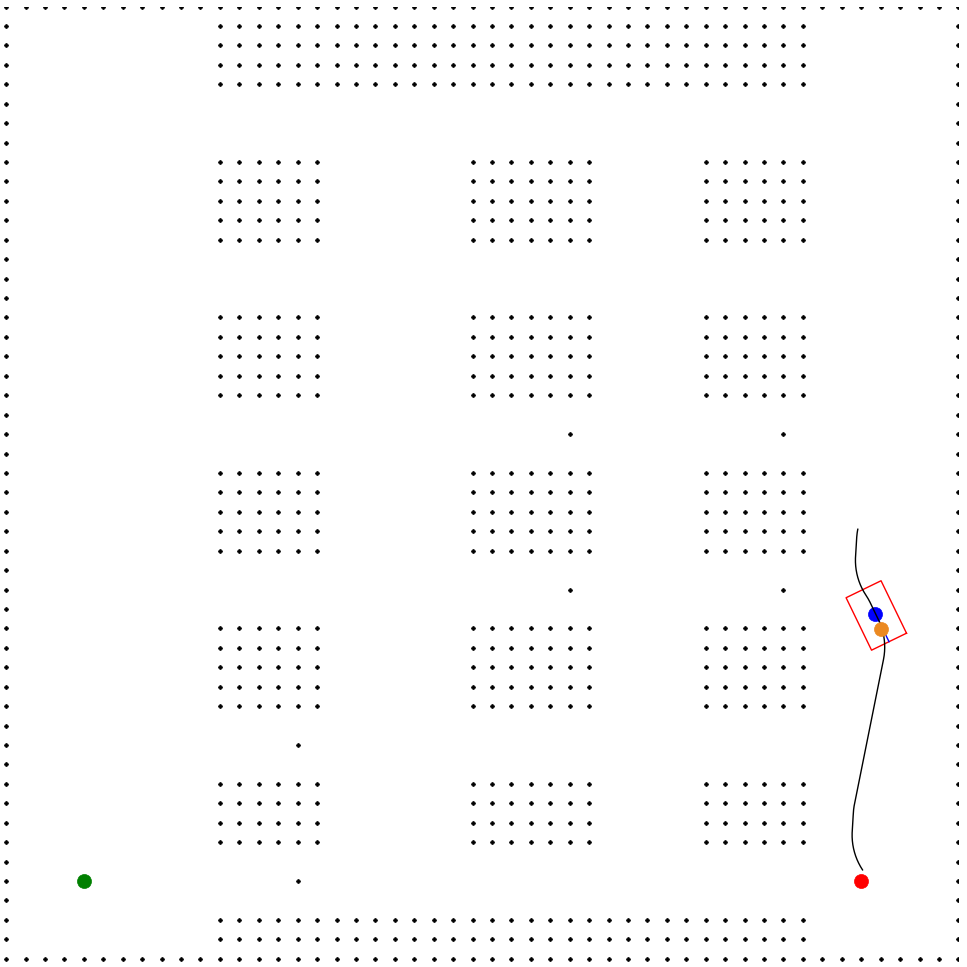
\includegraphics[width = \textwidth]{map6plan3_4.png}
        \caption{Replan 4}
        \label{fig:map65}
    \end{subfigure}
    \caption{Map 6 Planning Sequence}
    \label{fig:map6good}
\end{figure}

Our approach performs quite poorly in some situations, due to the fact that we have a small set of motion primitives. In cases where we get stuck in twisty, maze-like corridors, our motion primitives are not short enough to facilitate an exit motion. Such an exit motion (Fig.~\ref{fig:stuck}) requires multiple sequences of reverses and short turns, and our lack of short turns means that we cannot plan our way out of such situations. Additionally, when we see an obstacle and are close to a wall, the lack of short primitives leads to planning failure, due to the lack of short primitives that would enable the robot to maneuver out of its tightly constrained position.

\begin{figure}[ht]
\centering
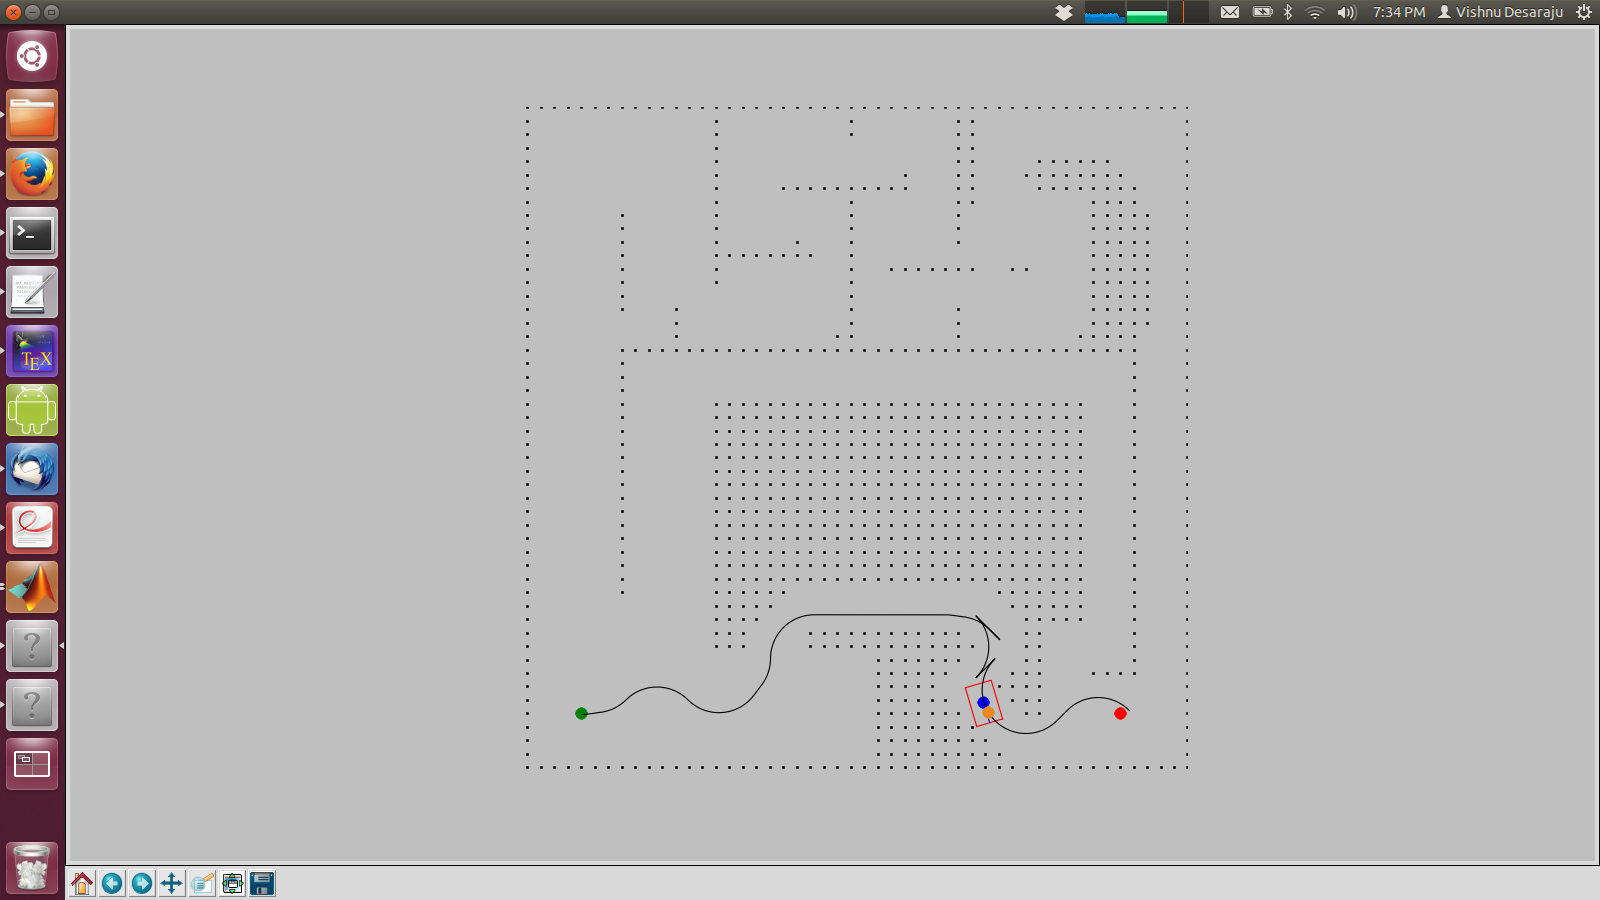
\includegraphics[width=128pt,keepaspectratio]{stuck_in_map2_S.png}
\caption{Planning Failure (Map 2)}
\label{fig:stuck}
\end{figure}

\newpage

Overall, the controller seems to track the trajectory of the robot well, but due to the heavily constrained dynamics of the robot (not being able to steer during reverse), even a slight offset in trajectory tracking can lead to collision/divergence, if a reverse primitive is part of the trajectory.

\end{document}

